
\begin{figure}[bt]
\centerline{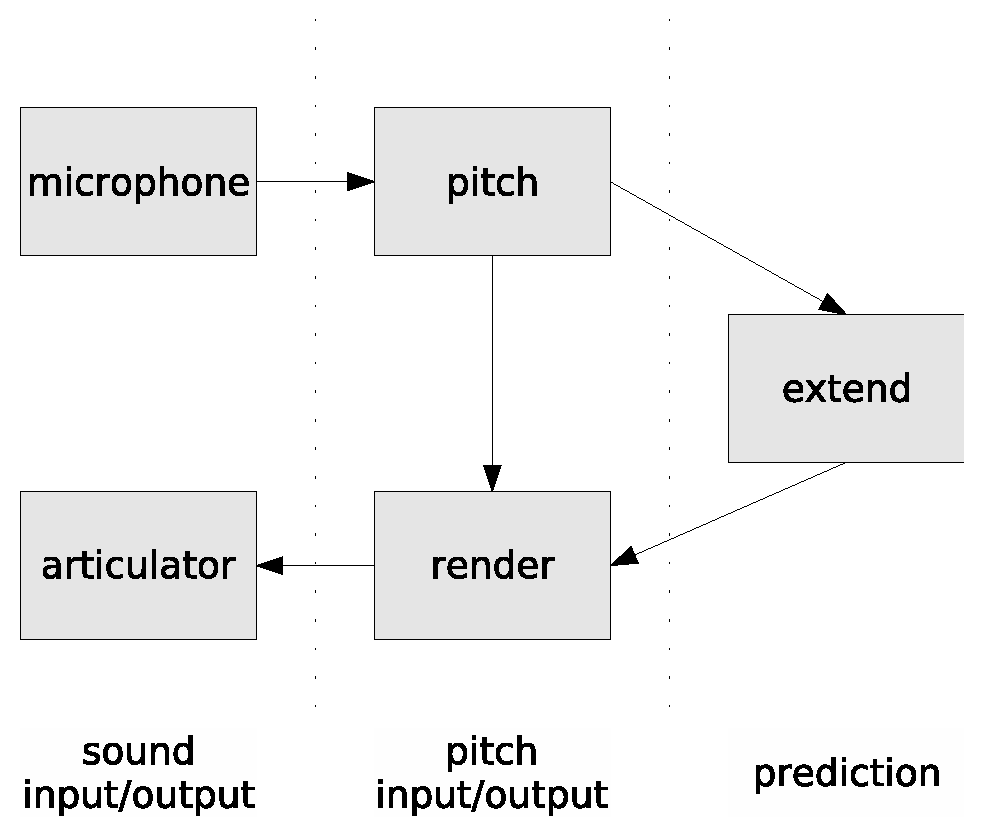
\includegraphics[height=6cm]{images/sing-modules}}
\caption {
%
\label{fig:sing-module}
%
The system for vocal interaction.
The behavior is implemented in the module labelled {\bf render} which
takes the output both of the pitch detector ({\bf pitch}) and a simultaneous 
prediction of what the pitch ``ought'' to be (from {\bf extend})
and decides what sound to make if any.
%
}
\end{figure}


\begin{figure}[bt]

\centerline{
a)
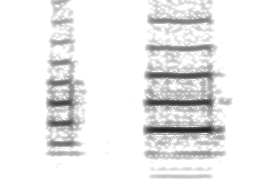
\includegraphics[height=2cm]{images/chico-output-separate-high-low}
\ \ 
\ \ 
b)
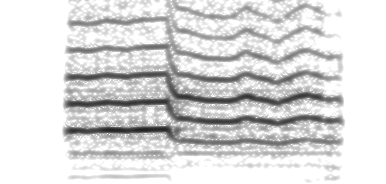
\includegraphics[height=2cm]{images/chico-output-pair-high-low}
\ \ 
\ \ 
c)

\includegraphics[height=2cm]{images/chico-output-ohm}
}

\caption{
%
\label{fig:singing-outcome}
%
During a single session the artifact was induced
to generate three distinch patterns of ``speech'': a) two separated
vocalizations with rising pitch; b) a single vocalization with
two tones of falling pitch; and c) a long vocalization of low, steady
pitch.
%
These spectrogram fragments are taken from one continuous session
with the artifact.  Fragments (a) and (b) are generated entirely
by the artifact; fragment (c) is overlaid by sound from
the human partner as well (it was a simultaneous ``meditative chant'').
%
}

\end{figure}





\begin{figure}[bt]

\centerline{(a$_1$) 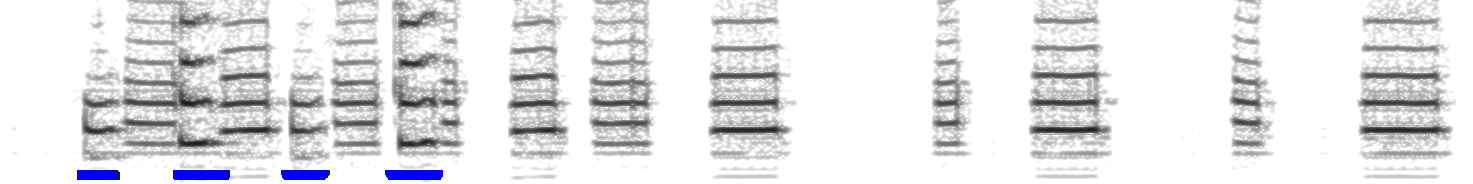
\includegraphics[height=2cm]{images/chico-separate-begin-labelled}}

\ \\

\centerline{(a$_2$) 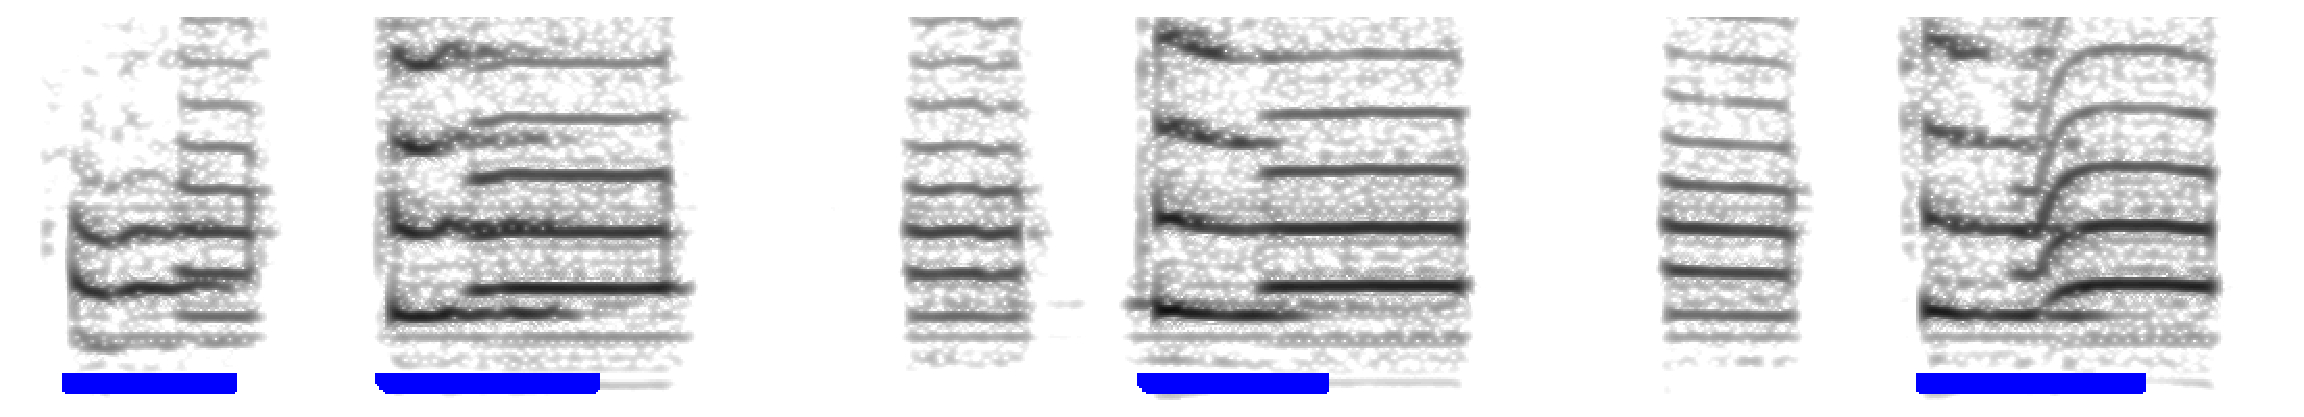
\includegraphics[height=2cm]{images/chico-separate-together-labelled}}

\ \\

\centerline{(c) 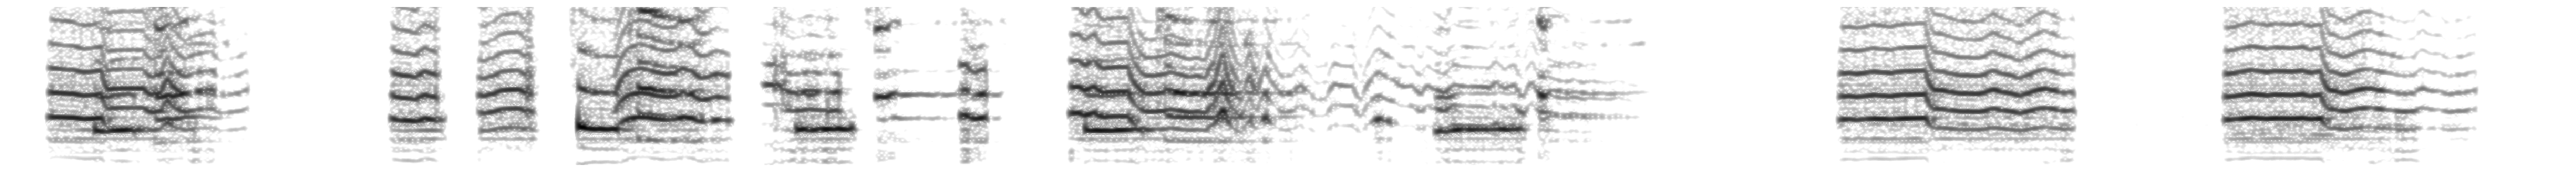
\includegraphics[height=1cm]{images/chico-pair}}

\ \\

\centerline{(d) 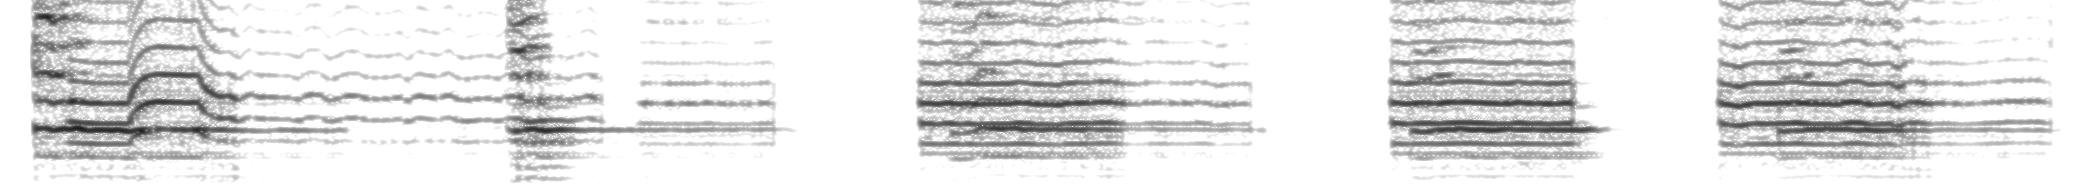
\includegraphics[height=1cm]{images/chico-ohm}}


\caption{
%
\label{fig:sing-spectrogram}
%
Sequence (a$_1$) is a spectrogram of the first 14 seconds of human/artifact 
interaction in a 54-second experiment. 
Since we are only concerned with pitch, the 
spectrogram is cropped to emphasis the vertical ``striping'' of 
horizontal lines that reflects the pitch (the greater 
the distance between stripes, the higher the frequency).
The blue bar at the bottom of the spectrogram is added to 
indicate when the human is vocalizing.
%
We see that the human initiates with a short vocalization
and the artifact responds with a short vocalization.  When it
finishes, the human makes a vocalization with a higher pitch.
The artifact responds with a vocalization with a higher pitch.
The human then repeats the first, lower, vocalization.
The artifact responds.  The human repeats the higher vocalization.
The artifact responds with a very abbreviated low tone, then a delay,
then the ``correct'' hight tone.  The human remains silent at this
point, and the robot starts generating a seqence of low and high
tones.
%
Sequence (a$_2$) follows on immediately from sequence (a$_1$), with 
the human ``joining in'', vocalizating at the same or overlapping time 
as the artifact.  The pattern of vocalization continues low-high,
low-high, like a very simple tune.
%
The tune has been introduced to the artifact without any
explicit or mandatory turn-taking.
%
Sequences (c) and (d) show periods within the same 54-second experiment
where the artifact's behavior is ``shaped'' in the same way
to produce two other tunes.
}

\end{figure}



\section{Participation in rhythmic events}

As a component of exploratory play, we are interested in giving our
robot the ability to participate in patterned activity in real time
with a human partner.  We include in principle any form of
coordinated motor activity, including vocalization
(singing, proto-dialogue), and gesturing (tapping, dancing).
%
For example, if a human starts humming or tapping something rhythmic, 
we'd like the robot to rapidly join in.
%
This goes beyond the strictly manipulation-based scenarios initially
envisaged for this deliverable, extending the scope to vocal interactions
as well.  By finding mechanisms that span the different motor systems,
we contribute to the overall goal of the embodied artifact work: to
find common sensorimotor mechanisms between between speech and 
manipulation.


Why is this particular form of interaction
useful?  Participation in rhythmic activity is a means to
an end, rather than a goal in itself.  The overall goal is to make
machine learning on our robots more autonomous.
%
Knowing the overall structure of an activity gives a ``skeleton'' upon
which the specific objects and actions (potentially initially
unmodeled) within that activity could be analysed.
%
Also, participating in activity is better than just observing it,
since there is an implicit signalling of ``comprehension'' level
available to the human partner, who can reasonably be expected to
adjust their behavior accordingly.


The theoretical mechanism was reported in deliverable 1.6.  
UGDIST has made a practical application of that mechanism to
vocal interaction, specifically, to a pitch perception/production
experiment.  We attached prediction to the property of acoustic pitch
as shown in Figure~\ref{fig:sing-module}.


Results of a 54-second ``singing'' experiment are shown in 
Figures \ref{fig:singing-outcome} and \ref{fig:sing-spectrogram}. 
%
The key property being tested was whether the artifact's 
``speech'' production could be shaped in real-time by
a human partner to match their own.
%
Further, we were testing whether this process could be
repeated multiple times (rather than being a once-off
process that requires a ``reset'').
%
In fact, within a minute, it proved possible to
coax the artifact to produce three stable vocalizations
(shown in Figure~\ref{fig:singing-outcome}).
%
When the vocalizations were produced, they were stable
regardless of whether the artifact produced them alone,
of if the human partner also produced all or part of them.
%
Moving from one stable vocalization to another 
took on the order of 15-20 seconds.

This shows that the theoretical method of sequence prediction can be
usefully applied in practice.  The next steps with this system should
be:

\begin{itemize}

\item To apply prediction across multiple features of speech.

\item To apply work to arm movements and gesturing.

\item To exploit the knowledge of the structure of an activity to
learn about the individual parts of that activity.

\end{itemize}


